\chapter{Plataformas de desarrollo}
\label{cap:capitulo3}

En este capítulo se describen en detalle las tecnologías empleadas durante el desarrollo de este proyecto, así como el lenguaje de programación y las librerías utilizadas.

\section{Lenguajes de programación}
\label{sec:programación}
\subsection{Python}
\label{sec:python}

Python \footnote{\url{https://www.python.org/}} es un lenguaje de programación de alto nivel \footnote{\url{https://www.tecnologia-informatica.com/lenguaje-de-alto-nivel-que-es-ejemplos/}} interpretado \footnote{\textbf{Lenguaje de programación interpretado}: Lenguaje en el que las implementaciones se ejecutan directamente, sin necesidad de compilar el programa ni generar código máquina del mismo.} que ha ganado gran popularidad en los últimos años gracias a su simplicidad, versatilidad y enfoque multiparadigma \footnote{\textbf{Multiparadigma:} soporta programación orientada a objetos, funcional y procedimental.}. Posee una extensa colección de librerías que facilitan el desarrollo de aplicaciones en áreas muy diversas.

En este \ac{TFG}, Python 3 se emplea para el desarrollo completo del código, utilizando diversas bibliotecas tanto para la creación de entornos de entrenamiento y prueba de modelos, como para la implementación de algoritmos de {DRL}.

\subsubsection{Pygame}
\label{sec:pygame}

Pygame \footnote{\url{https://www.pygame.org/docs/}} es una librería de Python ampliamente utilizada para el desarrollo de juegos y aplicaciones multimedia. Proporciona un conjunto de herramientas que permite crear gráficos, visualizar imágenes y gestionar animaciones de manera sencilla y eficiente. Además, Pygame ofrece funcionalidades para la captura y el manejo de eventos de entrada, como las pulsaciones de teclas y los clics del ratón.

\begin{code}[h]
\begin{lstlisting}[language=Python]
	 import pygame
	
	# Setup
	pygame.init()
	screen = pygame.display.set_mode(size, pygame.HWSURFACE | pygame.DOUBLEBUF)
	pygame.display.set_caption(name)

	while True:
	    for event in pygame.event.get():
	        if event.type == pygame.QUIT:
	            pygame.quit()
	            break

	    screen.fill("purple") # Fill the screen with a color
	    pygame.display.flip() # Display your work on the screen

\end{lstlisting}
\caption[Ejemplo de código en Python utilizando Pygame]{Ejemplo de código en Python utilizando Pygame para mostrar una interfaz gráfica}
\label{cod:pygame}
\end{code}

 En este caso, se ha utilizado Pygame para desarrollar la interfaz gráfica del proyecto, permitiéndonos visualizar la nube de puntos del \ac{LiDAR} y las imágenes de las cámaras, así como su tratamiento, como el carril detectado o la clasificación de objetos.

\begin{figure}[ht]
  \begin{center}
    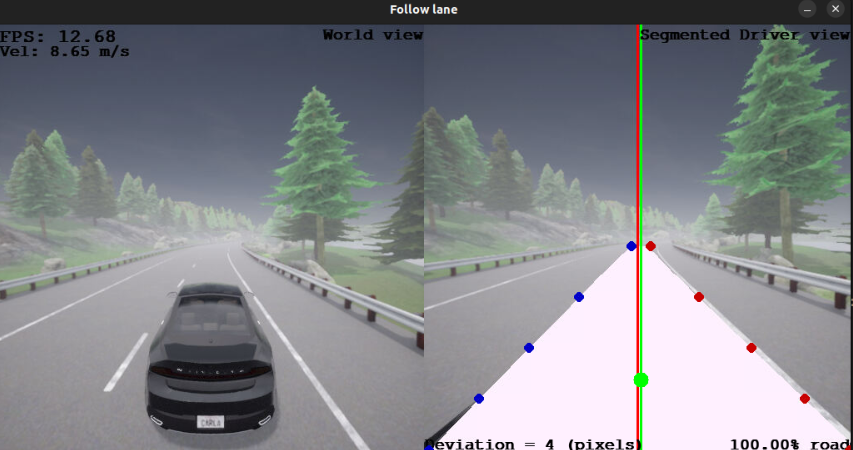
\includegraphics[width=9cm]{figs/Plataformas_Desarollo/pygame.png}
  \end{center}
  \caption{Interfaz gráfica desarrollada con Pygame.}
  \label{foto_pygame}
\end{figure}

\subsubsection{NumPy}
\label{sec:numpy}

NumPy \footnote{\url{https://numpy.org/}} es una librería de Python que proporciona soporte para matrices y ofrece una extensa colección de funciones matemáticas y operaciones optimizadas para trabajar con estos arreglos. Es ampliamente utilizada por su eficiencia computacional y facilidad de uso. En este proyecto, ha sido particularmente útil para manejar las matrices de imágenes y los \textit{arrays} utilizados para clasificar los datos del \ac{LiDAR}, permitiéndonos analizar y filtrar estos datos de manera eficiente.

\begin{code}[h]
\begin{lstlisting}[language=Python]
import numpy as np

index = np.argwhere(self._mask == ROAD)
index_sorted = index[np.argsort(index[:, 0])] # Sorted by y

\end{lstlisting}
\caption[Ejemplo de indexación y ordenación de datos con NumPy]{Ejemplo de indexación y ordenación de datos con NumPy}
\label{cod:numpy}
\end{code}

\subsubsection{Matplotlib}
\label{sec:plot}

La librería Matplotlib \footnote{\url{https://matplotlib.org/}} es una herramienta popular en Python para crear gráficos y visualizaciones. Permite generar desde gráficos simples hasta complejos, como líneas, barras, histogramas y diagramas de dispersión. Es ampliamente utilizada gracias a su flexibilidad para personalizar los gráficos y su integración con otras librerías como NumPy y Pandas \footnote{\url{https://pandas.pydata.org/}}, librería de Python para la manipulación y análisis de datos. Además, ofrece la posibilidad de exportar los gráficos en diversos formatos.

\begin{code}[h]
\begin{lstlisting}[language=Python]
import numpy as np
import matplotlib.pyplot as plt

# Crear un rango de valores para x
x = np.linspace(0, 2 * np.pi, 1000)

# Calcular los valores de seno y coseno para cada valor de x
y_seno = np.sin(x)
y_coseno = np.cos(x)

# Crear plots
plt.plot(x, y_seno, label='Seno', color='blue')
plt.plot(x, y_coseno, label='Coseno', color='red')

plt.title('Funciones Seno y Coseno')
plt.xlabel('x')
plt.ylabel('Valor')
plt.legend()
plt.grid(True)

# Mostrar plot
plt.show()
\end{lstlisting}
\caption[Ejemplo de cómo graficar las funciones seno y coseno con Matplotlib]{Ejemplo de cómo graficar las funciones seno y coseno con Matplotlib.}
\label{cod:plot}
\end{code}

\begin{figure}[ht]
  \begin{center}
    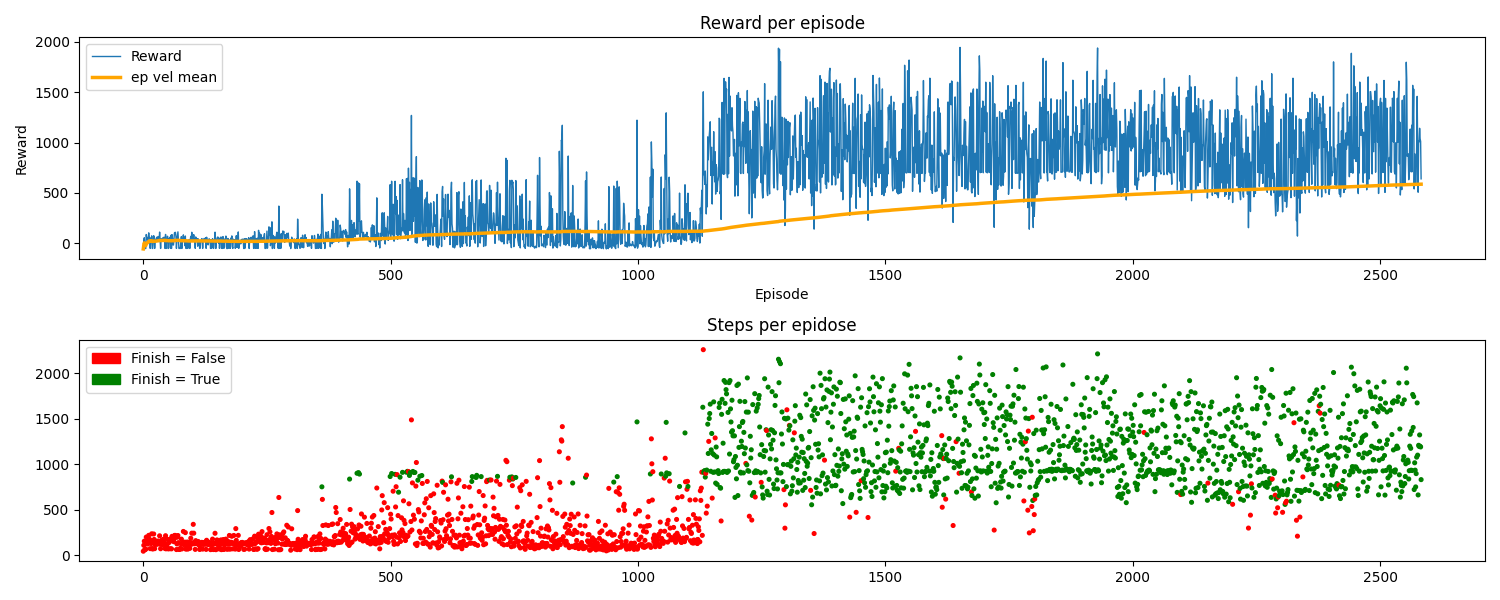
\includegraphics[width=6cm]{figs/Plataformas_Desarollo/plot.png}
  \end{center}
  \caption{Gráfico de las funciones seno y coseno con Matplotlib.}
  \label{foto_plot}
\end{figure}

En este \ac{TFG}, se ha utilizado principalmente la librería Matplotlib para la visualización de los datos recopilados durante la inferencia y a lo largo de los entrenamientos.

\subsubsection{Gymnasium}
\label{sec:gymnasium}

Gymnasium \footnote{\url{https://pypi.org/project/gymnasium/}}  es una biblioteca de Python desarrollada por OpenAI \footnote{\url{https://openai.com//}}  que proporciona herramientas para crear una amplia variedad de entornos, diseñados específicamente para aplicar y probar algoritmos de aprendizaje por refuerzo.

En nuestro proyecto de conducción autónoma, hemos utilizado la biblioteca Gymnasium, combinada con el simulador Carla, para crear los entornos de entrenamiento y prueba de nuestro modelo. Para ello, es necesario definir una clase personalizada que herede de la clase base \textit{Env} proporcionada por Gymnasium. En esta clase, configuramos las variables necesarias, como el espacio de observaciones, e implementamos los métodos fundamentales para el entrenamiento, \textit{step}, \textit{reset} y \textit{close}. A continuación, se muestra un ejemplo básico de implementación en Python:

\begin{code}[h]
\begin{lstlisting}[language=Python]

import gymnasium as gym

class CarlaBase(gym.Env):
    def __init__(self):
        self.observation_space = obs_space
    
    def _get_obs(self):
        return obs
    
    def _get_info(self):
        return info
    
    def step(self, action: np.ndarray):
        return self._get_obs(), reward, terminated, truncated, self._get_info()
   
    def reset(self, seed=None):
        return self._get_obs(), self._get_info()
    
    def close(self):
        # destroy carla actors
        pygame.quit()

\end{lstlisting}
\caption[Definición de un entorno personalizado en Gymnasium]{Definición de un entorno personalizado con Gymnasium.}
\label{cod:gym}
\end{code}

El espacio de observaciones es una descripción formal que define el tipo, la estructura y los límites de los datos que el agente puede recibir del entorno en cada momento. Funciona como un marco que delimita la información accesible para el agente. En Gymnasium, este espacio se configura mediante clases predefinidas, como \textit{Box}, \textit{Discrete} o \textit{Dict}, que establecen el rango permitido y la estructura de los datos. Esta configuración debe ser compatible con la política del modelo de aprendizaje utilizado, ya que define la entrada que la red neuronal o algoritmo de decisión del agente manejará. En nuestro caso, como utilizaremos una política basada en diccionarios, crearemos el espacio de observaciones continuo mediante la clase \textit{Dict}, que permite combinar múltiples espacios de observación en una estructura organizada.

\begin{code}[h]
\begin{lstlisting}[language=Python]

self.observation_space = spaces.Dict(
	spaces={
		KEY_CM: spaces.Box(
			low=0,
			high=SIZE_CAMERA - 1,
			shape=(2,),
			dtype=np.int32
		),
		KEY_LEFT_POINTS: spaces.Box(
			low=0,
			high=SIZE_CAMERA - 1,
			shape=(self._num_points_lane, 2),
			dtype=np.int32
		)
	}
)


\end{lstlisting}
\caption[Definición del espacio de observaciones en un entorno Gymnasium]{Definición del espacio de observaciones en un entorno Gymnasium.}
\label{cod:gymobs}
\end{code}

Los métodos \textit{step} y \textit{reset} son esenciales para ejecutar un algoritmo de aprendizaje por refuerzo, ya que permiten la interacción entre el agente y el entorno. La función \textit{step} recibe como entrada la acción tomada por el agente y devuelve una tupla con las nuevas observaciones del entorno, la recompensa obtenida, indicadores de si el episodio ha terminado o ha sido truncado y un diccionario con información adicional. Por otro lado, la función \textit{reset} se utiliza al comienzo de cada episodio para reiniciar el entorno a su estado inicial, devolviendo la primera observación y la información asociada. Juntos, estos métodos estructuran el ciclo iterativo de simulación, asegurando consistencia en el entrenamiento y permitiendo al agente aprender y mejorar su desempeño a lo largo de múltiples episodios.

\subsubsection{Stable Baselines 3}
\label{sec:stable_baselines3}

Stable-Baselines3 \footnote{\url{https://stable-baselines3.readthedocs.io/en/master/}} es una biblioteca de Python que nos proporciona implementaciones estables y fáciles de usar de algoritmos de aprendizaje por refuerzo basadas PyTorch \footnote{\url{https://pytorch.org/}} como \textit{backend}. Además, incluye compatibilidad con TensorBoard \footnote{\url{https://www.tensorflow.org/tensorboard?hl=es-419}}, lo que permite visualizar métricas del entrenamiento en tiempo real y analizar el rendimiento de los modelos. Entre las características principales de Stable-Baselines3 se encuentran tres tipos de políticas que permiten adaptar el modelo a diferentes tipos de datos:

 \begin{itemize} 
\item \textit{MlpPolicy:} Diseñada para trabajar con estados en forma de vectores, como en el entorno \texttt{CartPole} \footnote{\url{https://gymnasium.farama.org/environments/classic_control/cart_pole/}}, el cual consiste un carro que sostiene un poste, cuyo objetivo es mantener el poste dentro de un cierto ángulo tanto tiempo como sea posible, moviéndose hacia la izquierda o hacia la derecha. 
\item \textit{CnnPolicy:} Diseñada específicamente para procesar estados representados como imágenes, siendo ideal para aplicaciones como videojuegos.
\item \textit{MultiInputPolicy:} Permite manejar observaciones más complejas organizadas en diccionarios, adecuadas para datos combinados. 
\end{itemize} 

\begin{code}[h] \begin{lstlisting}[language=Python] 
from stable_baselines3.common.env_util import make_vec_env, PPO

# Instanciar entorno
env = make_vec_env(lambda: CarlaBase (), n_envs=1) 

 # Creacion y configuracion del modelo
model = PPO(policy, env, verbose=verbose, tensorboard_log=log_dir, **model_params)

# Entrenamiento
model.learn(total_timesteps=n_timesteps, log_interval=log_interval, tb_log_name=log_name, progress_bar=True) 

env.close()
model.save(model_name) # Salvar modelo
model = PPO.load(model_file, env=env, **new_model_params) # Cargar modelo
\end{lstlisting}
\caption[Ejemplo de código con Stable-Baselines3]{Entrenamiento de un modelo \ac{PPO} con la biblioteca Stable-Baselines3.} 
\label{cod:sb3} \end{code} 

El flujo general del entrenamiento con Stable-Baselines3 sigue una serie de pasos bien definidos: creación del entorno, configuración del modelo y entrenamiento. En primer lugar, al crear el entorno, debemos especificar la clase del entorno y el número de instancias (\textit{n\_env}), que en este caso será una sola. A continuación, creamos el modelo indicando el entorno utilizado, la política, el número total de \textit{steps} que durará el entrenamiento, así como otros parámetros de entrenamiento que se deseen ajustar. Si no se establecen valores específicos, se utilizarán los predeterminados.

El entrenamiento del modelo se lleva a cabo mediante la función \textit{learn}, que primero ejecuta la función \textit{reset}definida en el entorno, y luego de forma continua ejecuta \textit{step} hasta que se completa un episodio, que se vuelve a ejecutar \textit{reset} y este proceso continúa hasta que finaliza el entrenamiento. Una vez completado, podemos guardar el modelo con la función \textit{save} y cargarlo para futuros reentrenamientos con la función \textit{load}.

Además, los parámetros \textit{verbose} y \textit{progress\_bar} permiten configurar la visualización de los datos de entrenamiento. Los parámetros adicionales están relacionados con la ubicación de almacenamiento y la frecuencia con la que se recopilan los datos de entrenamiento para su posterior visualización con TensorBoard.

\begin{code}[h]
\begin{lstlisting}[language=bash]

tensorboard --logdir=$DIR

\end{lstlisting}
\caption[Comando para visualizar los datos en TensorBoard]{Comando para visualizar los datos con TensorBoard.}
\label{cod:cmdtsb}
\end{code}

\begin{figure}[ht]
  \begin{center}
    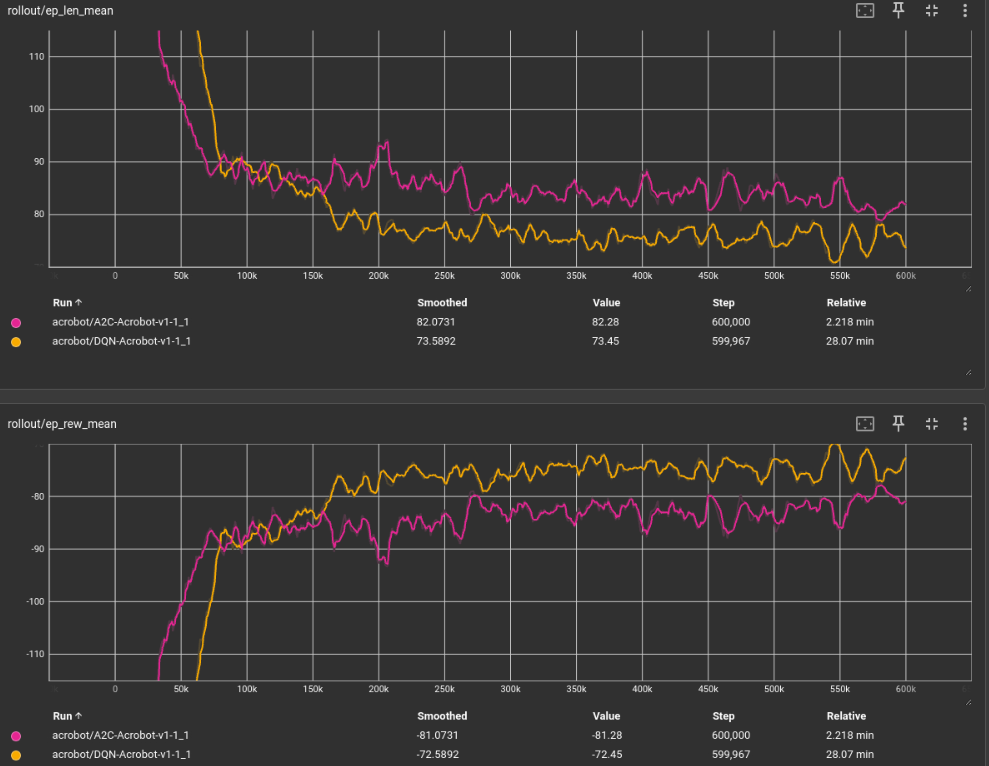
\includegraphics[width=7cm]{figs/Plataformas_Desarollo/TensorBoard.png}
  \end{center}
  \caption{Visualización de datos en TensorBoard.}
  \label{tensorboard}
\end{figure}

\section{Entornos de desarrollo}
\label{sec:des}

\subsection{Anaconda}
\label{sec:conda}

Anaconda \footnote{\url{https://www.anaconda.com/}} es una plataforma de distribución de software que facilita la gestión de entornos y bibliotecas para el desarrollo de aplicaciones en Python. Permite crear entornos aislados con versiones específicas de Python y otras dependencias, lo que ayuda a evitar conflictos entre proyectos y a garantizar que las aplicaciones se ejecuten con las versiones requeridas de las bibliotecas. En este \ac{TFG}, se crea un entorno Anaconda que nos permita utilizar la versión 3.10 de Python, ya que es la que necesitaremos para utilizar EfficientVit.

\begin{code}[h]
\begin{lstlisting}[language=bash]

conda create -n tfg python=3.10
conda activate tfg

\end{lstlisting}
\caption[Creación del entorno Anaconda]{Creación y activación del entorno Anaconda.}
\label{cod:anaconda}
\end{code}

\subsection{Visual Studio Code}
\label{sec:vs_code}

Visual Studio Code \footnote{\url{https://code.visualstudio.com/}} es un editor de código gratuito y compatible con varias plataformas, diseñado para crear, modificar y depurar código en varios lenguajes de programación. Este software también incluye herramientas adicionales como extensiones que optimizan la escritura en diferentes lenguajes, autocompletado de código y terminales integrados para hacer más eficiente la ejecución y depuración.

\begin{figure}[ht]
  \begin{center}
    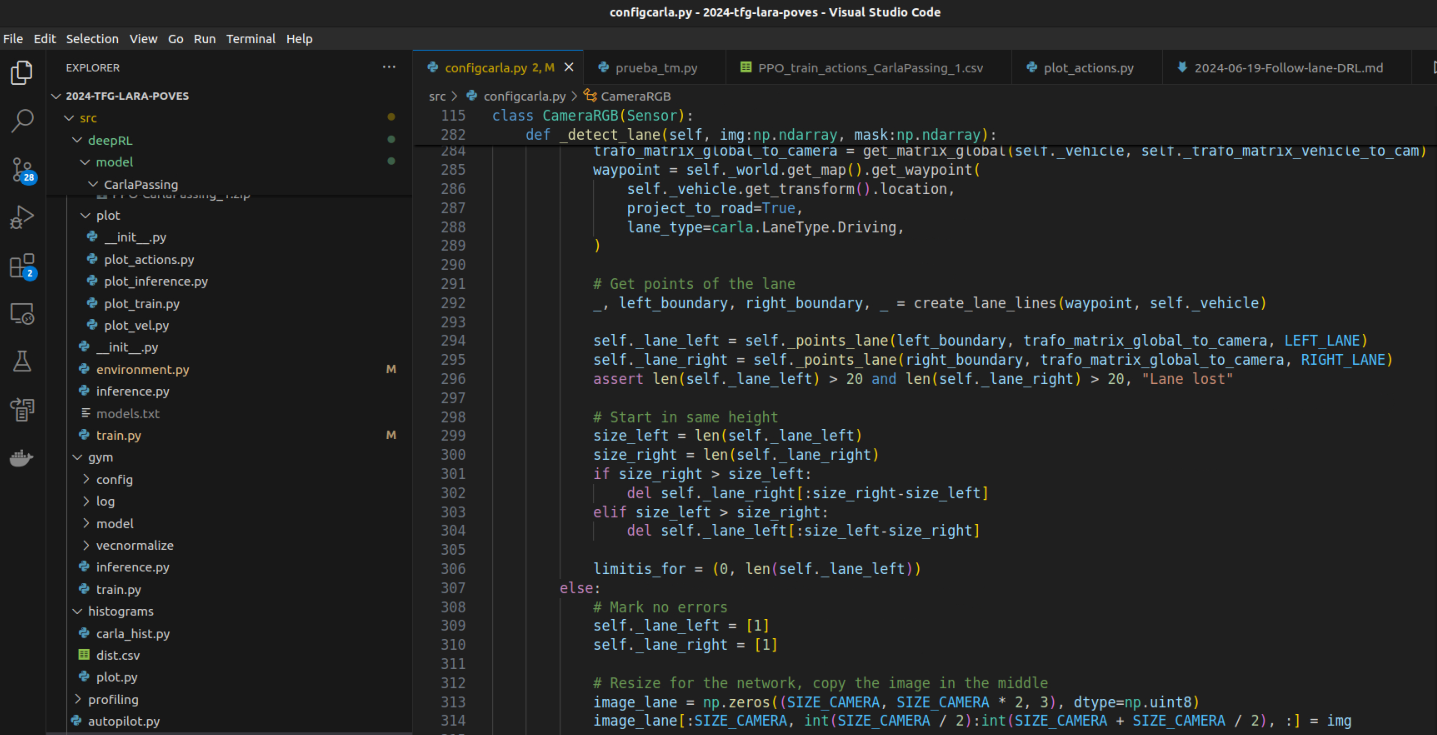
\includegraphics[width=12cm]{figs/Plataformas_Desarollo/visual_code.png}
  \end{center}
  \caption{Desarrollo en Visual Studio Code.}
  \label{foto_code}
\end{figure}

En este \ac{TFG}, se utiliza Visual Studio Code como el editor principal para el desarrollo de todo el código, aprovechando sus extensiones para Python y YAML \footnote{\url{https https://www.ibm.com/es-es/topics/yaml}}, lo que optimiza la productividad y facilita la escritura del código.

\section{EfficientVit}
\label{sec:ef}

\section{Entorno de simulación}
\label{sec:sim}
\subsection{CARLA}
\label{sec:carls}

Carla \footnote{\url{https://github.com/carla-simulator/carla}} un entorno de simulación de código abierto que se emplea en aplicaciones de vehículos autónomos y conducción asistida. Carla se basa en \textit{Unreal Engine de Epic Games} \footnote{\url{https://www.unrealengine.com/en-US}}, lo que le permite generar entornos urbanos y rurales altamente detallados y realistas. Estos entornos son ideales para simular la interacción de los vehículos autónomos con el entorno, probando su capacidad de navegación, toma de decisiones y respuesta ante situaciones imprevistas.

\begin{code}[h]
\begin{lstlisting}[language=bash]

/opt/carla/CarlaUE4.sh -world-port=2000

\end{lstlisting}
\caption[Comando para lanzar el simulador CARLA]{Comando para lanzar el simulador CARLA.}
\label{cod:cmdcarla}
\end{code}

Este simulador destaca por su capacidad de recrear escenarios dinámicos con una amplia variedad de condiciones de tráfico, clima y paisajes urbanos, lo que lo convierte en una herramienta poderosa para la investigación en condiciones similares a las del mundo real. Para aprovechar estos entornos, utilizaremos \textit{scripts} de Python que nos permitirán personalizar las simulaciones, brindando flexibilidad para ajustar propiedades como el comportamiento de los vehículos o la configuración de los sensores.

\begin{figure}[ht]
  \begin{center}
    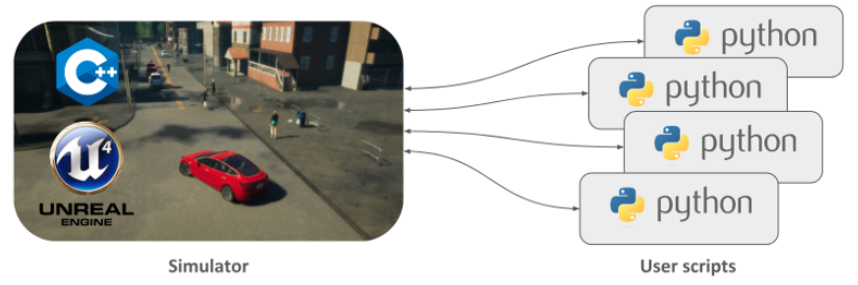
\includegraphics[width=9cm]{figs/Plataformas_Desarollo/carla.png}
  \end{center}
  \caption{Simulador CARLA.}
  \label{carla}
\end{figure}

En CARLA, los mapas son modelos tridimensionales detallados de ciudades y sus infraestructuras viales, que no solo incluyen la geometría de las carreteras y edificios, sino también objetos interactivos como semáforos, señales de tráfico y otros elementos estáticos, los cuales pueden activarse o desactivarse según las necesidades del simulador, permitiendo un alto grado de personalización. CARLA ofrece una amplia selección de mapas predefinidos que se pueden cargar directamente. Por otro lado, el mundo en CARLA se refiere al entorno completo de la simulación, que incluye el mapa, el clima, el tiempo, los vehículos, los peatones y otros elementos dinámicos, lo que permite crear una simulación realista, modificable en tiempo real para ajustar factores como la hora del día, las condiciones climáticas o el tráfico.

\subsubsection{Actores}

Los actores en CARLA son los elementos que realizan acciones dentro de la simulación y pueden interactuar con otros actores. Existen varios tipos de actores, cada uno con funcionalidades específicas:


\begin{itemize}
    \item \textit{Sensores.} Los sensores \footnote{\url{https://carla.readthedocs.io/en/latest/core_sensors/}} son actores que producen un flujo de datos. La mayoría de los sensores se adjuntan a un vehículo para recopilar información sobre su entorno. Existen varios tipos de sensores en CARLA. Los sensores escuchan datos y, cuando reciben información, llaman a una función descrita mediante una expresión \textit{Lambda} \footnote{\url{https://docs.python.org/3/reference/expressions.html}}. 

	\begin{code}[h]
	\begin{lstlisting}[language=python]
	
	camera_bp = blueprint_library.find('sensor.camera.rgb')
	camera = world.spawn_actor(camera_bp, transform, attach_to=vehicle)
	camera.listen(lambda image: image.save_to_disk('output/%06d.png' % image.frame))

	\end{lstlisting}
	\caption[Configuración de cámara RGB en CARLA]{Configuración de cámara RGB en CARLA.}
	\label{cod:camara_carla}
	\end{code}

    \item \textit{Espectador.} El espectador  proporciona un punto de vista dentro de la simulación. Puede utilizarse para mover la vista en la ventana del simulador.
    \item \textit{Señales de tráfico y semáforos.} En CARLA, solo las señales de alto, ceda el paso y los semáforos son considerados actores.

    \item  \textit{Vehículos.} Los vehículos en CARLA son un tipo especial de actor que simula la física de los vehículos de ruedas mediante componentes internos. Utilizan un controlador que define los atributos físicos del vehículo y otro que gestiona los comandos de conducción: aceleración, dirección y freno. CARLA ofrece varios tipos de vehículos (coches, motocicletas y camiones... \footnote{\url{https://carla.readthedocs.io/en/latest/catalogue_vehicles/}}), además de una gran variedad de modelos. El vehículo que se desea controlar, al que se le añaden los sensores, conocido como \textit{Ego Vehicle}, será el agente en el proceso de aprendizaje. Si indicamos esta condición al simulador, este renderiza solo la zona cercana a este vehículo para optimizar recursos.
	\begin{code}[h]
	\begin{lstlisting}[language=python]
	
	vehicle_vp = world.get_blueprint_library().find(vehicle_type)
	vehicle_vp.set_attribute('role_name', 'hero') # Ego vehicle
	ego_vehicle = world.spawn_actor(vehicle_bp, transform)
	ego_vehicle.apply_control(carla.VehicleControl(throttle=0.5, steer=0.1, brake=0.01))

	\end{lstlisting}
	\caption[Configuración de \textit{Ego Vehicle} en CARLA]{Configuración de \textit{Ego Vehicle} en CARLA.}
	\label{cod:ego_carla}
	\end{code}
    \item \textit{Peatones.} Los peatones funcionan de manera similar a los vehículos. El control sobre ellos se proporciona mediante controladores.
\end{itemize}

\subsubsection{Traffic Manager}

El \ac{TM} es el módulo encargado de controlar los vehículos en modo piloto automático dentro de una simulación. Su propósito principal es recrear condiciones de tráfico urbano realistas en el entorno simulado. Los usuarios tienen la posibilidad de personalizar ciertos comportamientos para configurar escenarios específicos de aprendizaje, lo que resulta esencial para entrenar sistemas de conducción bajo circunstancias particulares.

El \ac{TM} está integrado en el lado cliente de CARLA, y es necesario especificar el puerto de conexión para su funcionamiento. Los usuarios pueden ajustar parámetros del flujo de tráfico, permitiendo, forzando o incentivando comportamientos específicos. Por ejemplo, se puede configurar que los vehículos ignoren los límites de velocidad, cambien de carril de forma obligatoria o adopten comportamientos personalizados. Estas capacidades permiten experimentar y simular situaciones esenciales para la formación y evaluación de sistemas de conducción autónoma.

En nuestro caso, los entrenamientos estarán limitados al uso del piloto automático para el coche delantero con una velocidad fija e ignorando completamente las señales de tráfico para realizar el control adaptativo el tráfico y el adelantamiento. 
\begin{code}[h]
	\begin{lstlisting}[language=python]
	
	tm = client.get_trafficmanager(port)
	vehicle.set_autopilot(True, tm.get_port())  
	tm.ignore_lights_percentage(vehicle, 100) 
	self._tm.set_desired_speed(vehicle, velocity) #km/h
\end{lstlisting}
\caption[Configuración del \ac{TM} en CARLA]{Configuración del \ac{TM} en CARLA.}
\label{cod:tm_carla}
\end{code}










